\hypertarget{Chap:Filtering}{%
\section{State Estimation}\label{Chap:Filtering}}

Consider the two robots given in \texttt{fig:robotsandhumans}. How
should we approach designing robots to function in conjunction with
humans or instead of humans? For example:

\begin{itemize}
\tightlist
\item
  Robotic system to move goods through a distribution center.
\item
  Robotic system to care for the elderly.
\item
  Robotic system to perform tasks in hostile environments (deep sea,
  reactors, space, underwater caves, etc).
\item
  Robotic systems for assistive technology.
\end{itemize}

To do this we need to have perception of a changing environment, we need
to make decisions about how to respond based on the robot function
(goals) and we need to control effectors to carry out the intended
functions. For robot perception alone, we scan the environment, segment
out objects and then recognize the objects. There many types of sensors
used to just understand the surrounding environment:

\begin{itemize}
\tightlist
\item
  Contact sensors
\item
  Internal Sensors
\item
  Accelerometers
\item
  Gyroscopes
\item
  Compasses
\item
  Proximity Sensors
\item
  Sonar
\item
  Radar
\item
  Laser range finders
\item
  Infrared
\item
  Cameras
\item
  GPS
\end{itemize}

One of the basic functions, localization, is completely dependent on the
sensors. Decisions about future actions are made based on the sensors.
Feedback from the actuators is also based on the sensors. Many aspects
of the system ride on the sensors. The Sensors Chapter presented a
number and variety of sensing systems. There is a vast array of sensors
which can sense or measure physical quantities. Accuracy on sensors
varies greatly with some very accurate and others having considerable
errors.

\begin{quote}
Examples of two robotics systems that interact with humans.
\end{quote}

\begin{figure}
\centering
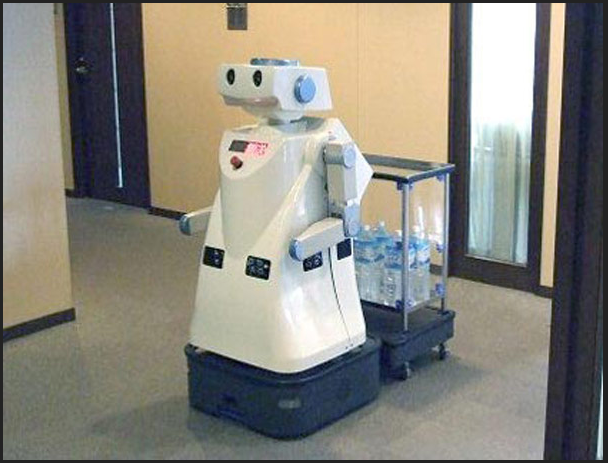
\includegraphics[width=0.4\textwidth,height=\textheight]{FilteringFigures/CartBot.png}
\caption{}
\end{figure}

\textbf{Problem}: How can we design a system which can function without
human input but has random elements in the environment? How can the
system determine its location accurately enough to navigate? How can the
robot use manipulators around humans safely if manipulator location,
feedback and control are uncertain. In manufacturing systems, we are
able to instrument objects of interest and highly constrain the
environment. The robot might not be local and the object to be
manipulated may have a known location. Clearly variation and noise
occur, but not to the degree found in robots that are intended to go
into the world and operate outside the confines of a factory.

All of tht said, observation is not the whole story. The robot will be
out observing the world, even though the observations often include
random noise, you normally have additional information that allows you
to remove significant noise. For example, if we are observing motion, we
know that not all types of motion will be possible. The basic laws of
physics clearly play a role. In addition the design and details of the
robot also play a role. These constrain the possibilities and in doing
so, help improve our estimates of the robot state.

StateEstimation SensorFusion ModelsandDynamicSystems KalmanFilters
ExtendedKalmanFilter Complementary Particle Filtering\_Problems
